\documentclass[a4paper, 14pt]{extarticle}
\usepackage{enumitem}
\usepackage{fefutitle}
\usepackage{xcolor}
\usepackage{amsmath}
\usepackage{graphicx}
\usepackage[justification=centering]{caption}
\usepackage{float}

\begin{document}
	\fefutitle{6}
	\pagebreak	

	\section{Введение}
		Уравнение переноса -- дифференциальное уравнение в частных производных, описывающее изменение скалярной величины в пространстве. Для численного решения таких уравнений существует несколько способов. Один из них, который будет использоваться в данной лабораторной работе -- метод частиц. Метод частиц состоит в представлении тела совокупностью взаимодействующих частиц(материальных точек), описываемых законами классической механики.
		
	\section{Создание математической модели}
		Пусть у нас есть $n$ частиц c начальными координатами $(x_i, y_i)$ и каждая частица обладает своей концентрацией:
		\[ C_i = C(x_i, y_i, t)\]
		
		В начальный момент времени: 
		\[ C_i = C(x_i, y_i, 0) \]
		
		И есть поле скорости $\psi = \psi(x, y)$ с компонентами скорости:
		\[ \begin{cases}
			u_x (x, y) = -\dfrac{\partial \psi}{\partial x} \\[7pt]
			\upsilon_y (x, y) = \phantom{-} \dfrac{\partial \psi}{\partial y}
		\end{cases} \]
		
		Таким образом, скорость частиц по осям OX и OY:
		\[ \begin{cases}
				\dfrac{dx_i}{dt} = u_x(x_i, y_i) = -\dfrac{\partial \psi}{\partial x}, \\[7pt]
				\dfrac{dy_i}{dt} =\upsilon_Y (x_i, y_i) = \phantom{-}\dfrac{\partial \psi}{\partial y}
			\end{cases}
		\]

	\section{Реализация модели}
		Начальные координаты точек задаём случайно от 0 до 1.
		
		За поле скорости возьмем следующую функцию:
		\[ \psi = \sin(2\pi x) \cdot \sin(\pi y) \]
		
		За функцию концентрации:
		\[ C(x, y, t) = C(y) = \arctan{\Bigg(\dfrac{y-0.5}{0.1}\Bigg)} \]
			
		Модель была реализована в Python.
		\begin{figure}[H]
			\begin{minipage}{0.5\textwidth}
				\centering
				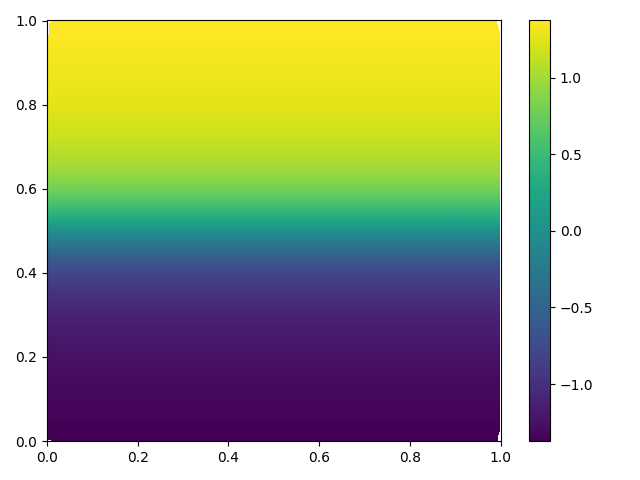
\includegraphics[width = \linewidth]{1.png}
			\end{minipage}\hfill
			\begin{minipage}{0.5\textwidth}
				\centering
				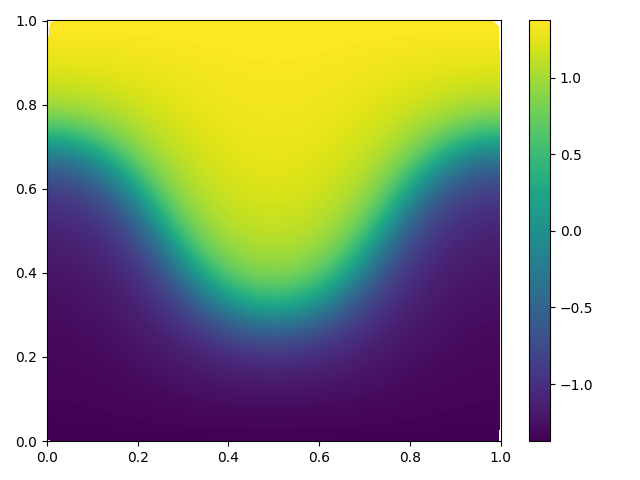
\includegraphics[width = \linewidth]{2.png}
			\end{minipage}\hfill
		\end{figure}
	
		\begin{figure}[H]
			\begin{minipage}{0.5\textwidth}
				\centering
				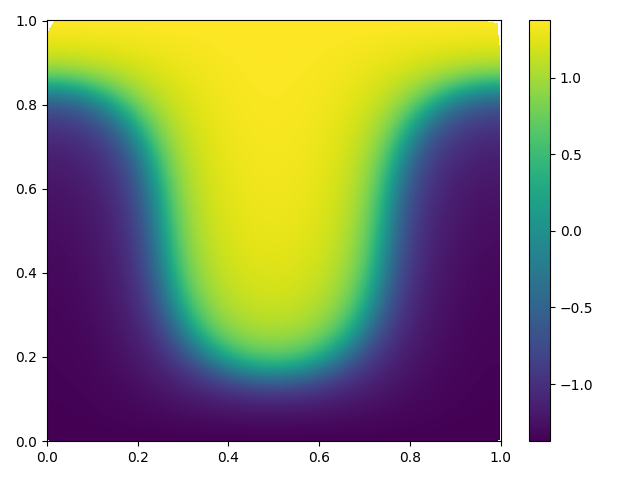
\includegraphics[width = \linewidth]{3.png}
			\end{minipage}\hfill
			\begin{minipage}{0.5\textwidth}
				\centering
				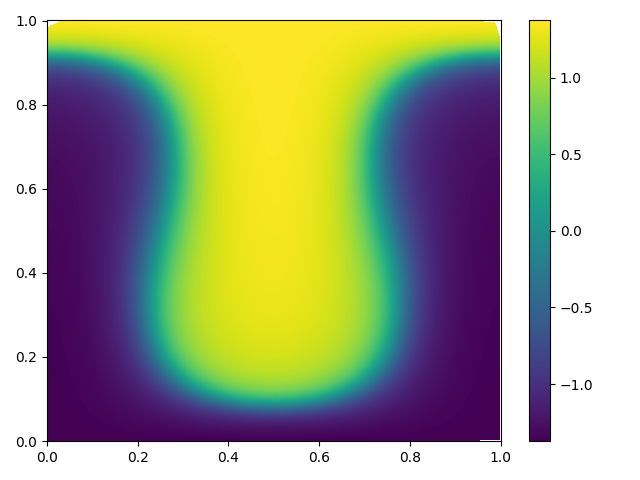
\includegraphics[width = \linewidth]{4.png}
			\end{minipage}\hfill
		\end{figure}
	
		\begin{figure}[H]
			\begin{minipage}{0.5\textwidth}
				\centering
				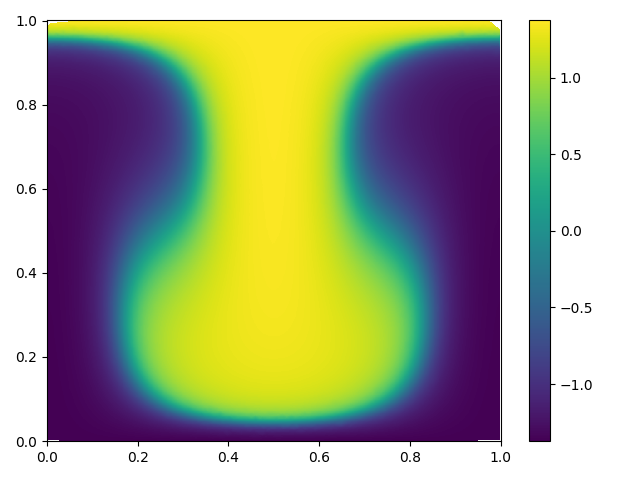
\includegraphics[width = \linewidth]{5.png}
			\end{minipage}\hfill
			\begin{minipage}{0.5\textwidth}
				\centering
				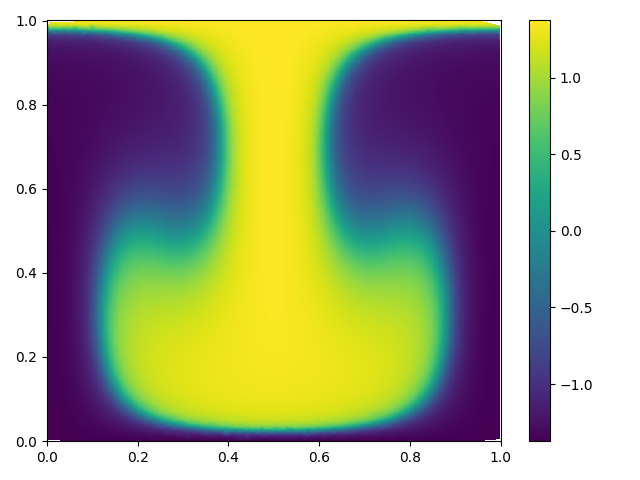
\includegraphics[width = \linewidth]{6.png}
			\end{minipage}\hfill
		\end{figure}
	
		\begin{figure}[H]
			\begin{minipage}{0.5\textwidth}
				\centering
				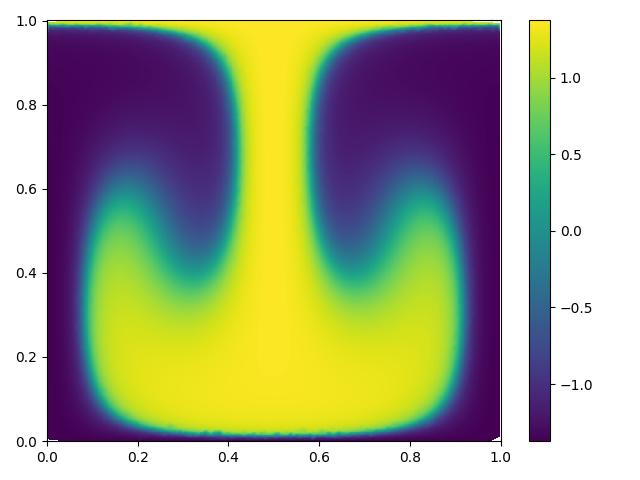
\includegraphics[width = \linewidth]{7.png}
			\end{minipage}\hfill
			\begin{minipage}{0.5\textwidth}
				\centering
				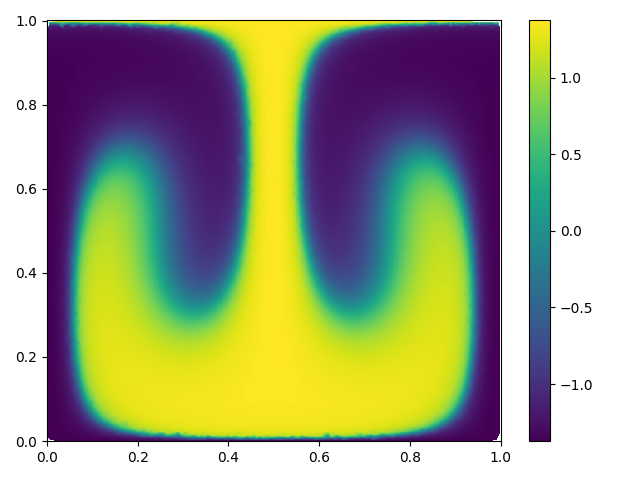
\includegraphics[width = \linewidth]{8.png}
			\end{minipage}\hfill
		\end{figure}
	
		\begin{figure}[H]
			\begin{minipage}{0.5\textwidth}
				\centering
				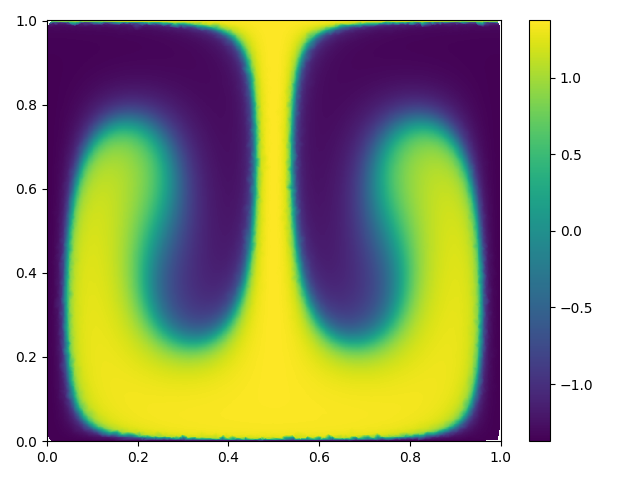
\includegraphics[width = \linewidth]{9.png}
			\end{minipage}\hfill
			\begin{minipage}{0.5\textwidth}
				\centering
				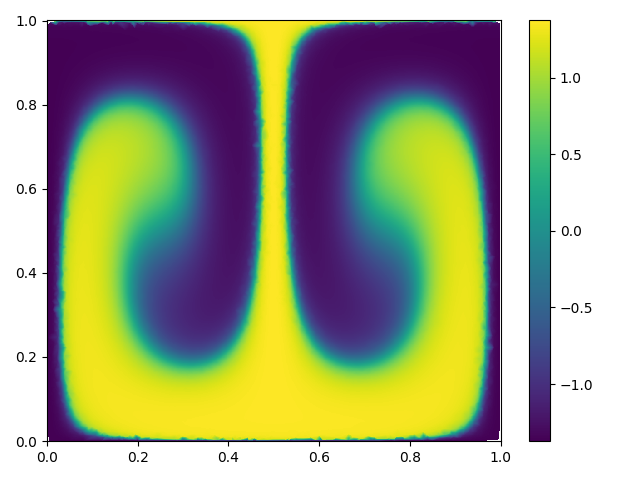
\includegraphics[width = \linewidth]{10.png}
			\end{minipage}\hfill
		\end{figure}
		
	\section{Вывод}
		
\end{document}	